\documentclass[a4paper,12pt]{article} % The document class with options

\usepackage[margin=1in]{geometry}
\usepackage{newtxtext,newtxmath}
\usepackage[T1]{fontenc}
\usepackage{amsmath}
\usepackage{amsfonts}
\usepackage{microtype}
\usepackage{graphicx}
% chktex-file 3
% chktex-file 18
% chktex-file 36
% chktex-file 44

\begin{document}
\setlength{\parskip}{1em} 
\setlength{\parindent}{0pt}
\newcommand{\vect}[1]{\mathbf{#1}}

\title{MECH 503 LAMMPS Project Report}
\author{Jincong Li \\ 60539939}
\date{\today}
\maketitle

\section*{Introduction}
Elastic constants are pivotal in understanding materials' responses to external forces, 
providing insights into stiffness and stability. With the advancement of molecular dynamics 
(MD) simulations, notably through the Large-scale Atomic/Molecular Massively Parallel Simulator
(LAMMPS), researchers can now predict these constants with high precision, bypassing the 
limitations of traditional experimental methods.

This study leverages LAMMPS to compute the elastic constant tensor for four 
materials: hexagonal close-packed magnesium (hcp-Mg), face-centered cubic aluminum 
(fcc-Al), body-centered cubic tungsten (bcc-W), and a novel face-centered cubic 
high-entropy alloy (HEA) consisting of nickel, iron, chromium, and cobalt. 
These materials are selected for their diverse applications, from aerospace to 
high-temperature environments. The focus is on examining the convergence of
the elastic constant tensor as a function of the finite difference displacement 
variable, "up" across a range from 0.01 to 0.0000001. This analysis is crucial for
validating the accuracy of our simulations against experimental and other 
computational data, providing a foundation for further exploration in materials science.

\section*{Methology}
\subsection*{Simulation Setup}
The molecular dynamics simulations were conducted using LAMMPS, focusing on four materials: hcp-Mg, fcc-Al, bcc-W, and an equiatomic high-entropy alloy of Ni, Fe, Cr, Co. For the high-entropy alloy, a Matlab script \texttt{make\_fcc\_random\_cell.m} was utilized to generate ten random FCC cells, ensuring a diverse representation of the alloy's microstructure. These cells were input into LAMMPS using the \texttt{read\_data} command.

\subsection*{Potential Models}
Interaction potentials were chosen based on their ability to accurately represent each material's physics:
\begin{itemize}
    \item hcp-Mg, fcc-Al, and bcc-W: Embedded Atom Method (EAM) potentials were employed, sourced from literature where parameters have been validated against experimental and \textit{ab initio} data.
    \item High-Entropy Alloy: The \texttt{eam/alloy} pair style was used with parameters from a comprehensive study ensuring the representation of complex multi-element interactions.
\end{itemize}

\subsection*{Finite Difference Parameter Analysis}
The elastic constant tensor's sensitivity to the finite difference displacement variable ``up'' was investigated by varying ``up'' between 0.01 to 0.0000001. This range was selected to encompass a broad spectrum of potential physical responses, enabling an assessment of convergence behavior. The analysis involved incrementally displacing atoms in the simulation cell and measuring the resultant stress, with elastic constants derived from the stress-strain relationship.

\subsection*{Data Processing and Analysis}
Post-simulation, the output data were processed using Python scripts to calculate the elastic constants from the stress-strain relationships. Convergence plots were generated for each material, highlighting how the calculated elastic constants stabilize as ``up'' decreases. Special attention was given to the high-entropy alloy, considering the random nature of its structure.

\subsection*{Comparison with Existing Data}
The obtained elastic constants were compared to available experimental data and previous computational studies, such as those by Mishin et al., for validation purposes. This comparison aimed to assess the accuracy of the MD simulations conducted in this study and to elucidate the potential impact of the chosen potentials and simulation parameters on the results.

\section*{Result}
\begin{table}[ht]
    \caption{Species, Lattice Format and Parameter(a) }
    \centering
    \begin{tabular}{|c|c|c|}
        \hline
        Species& Lattice &a \\
        \hline   
        Al & fcc & 4.05[1] \\
        Mg & hcp & 3.21[2]\\
        W & bcc & 3.165[1]\\
        \hline
    \end{tabular}
\end{table}

\begin{figure}[ht]
    \centering
    \includegraphics[width=1.1\textwidth]{Al.png}
    \caption{Convergence for Components of the Elastic Constant Tensor for fcc Al}
\end{figure}

\begin{figure}[ht]
    \centering
    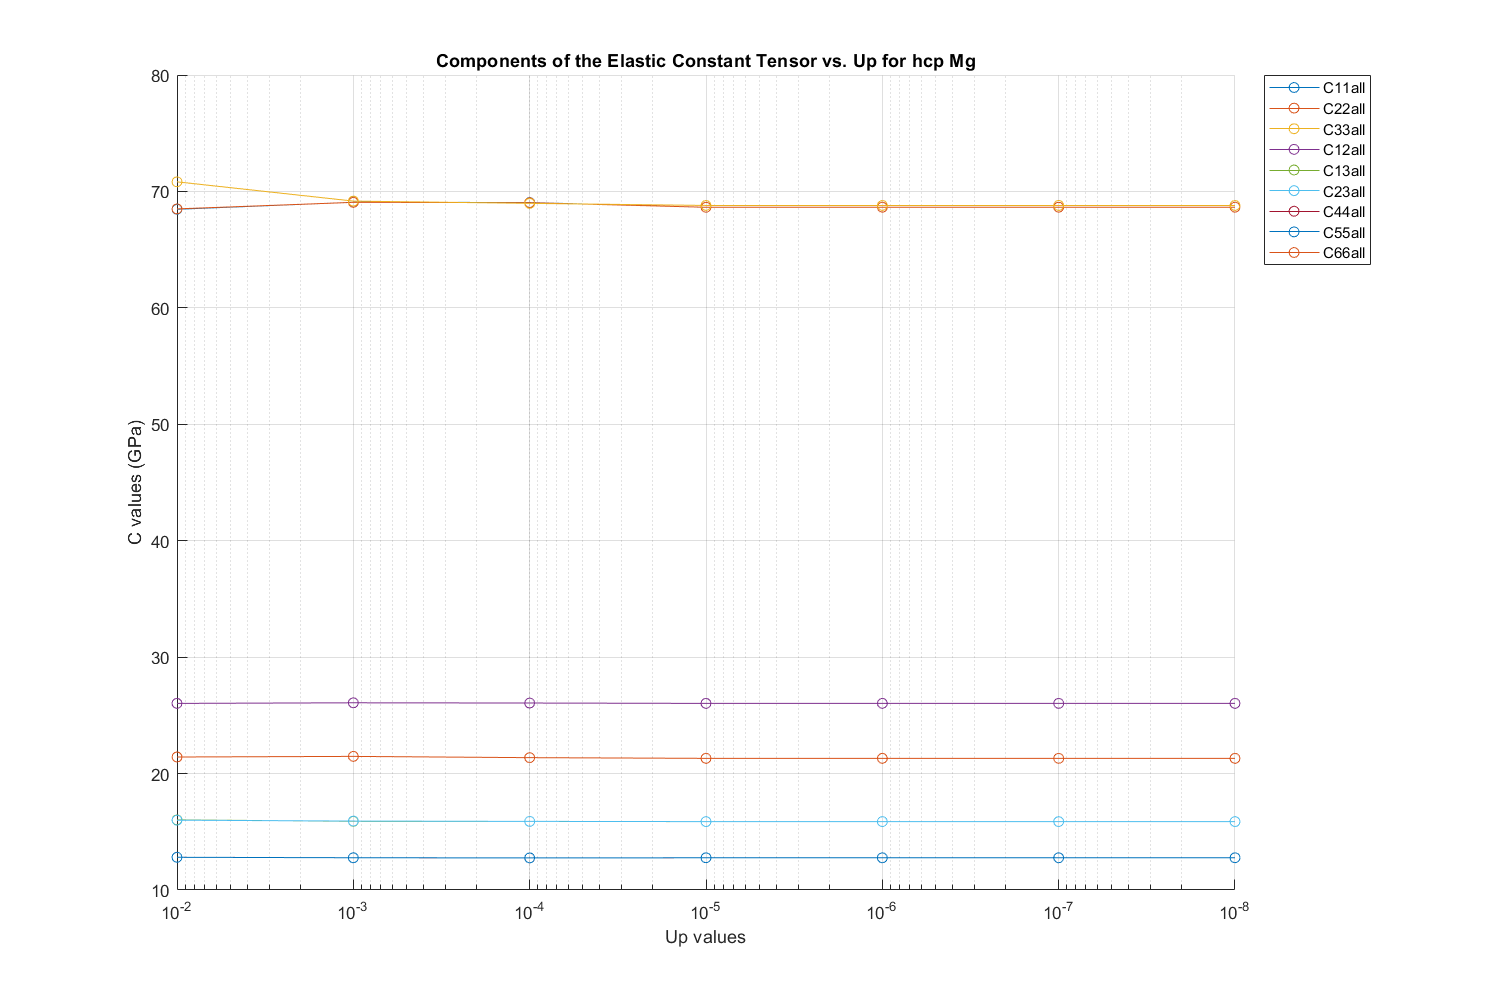
\includegraphics[width=1.1\textwidth]{Mg.png}
    \caption{Convergence for Components of the Elastic Constant Tensor for hcp Mg}
\end{figure}

\begin{figure}[ht]
    \centering
    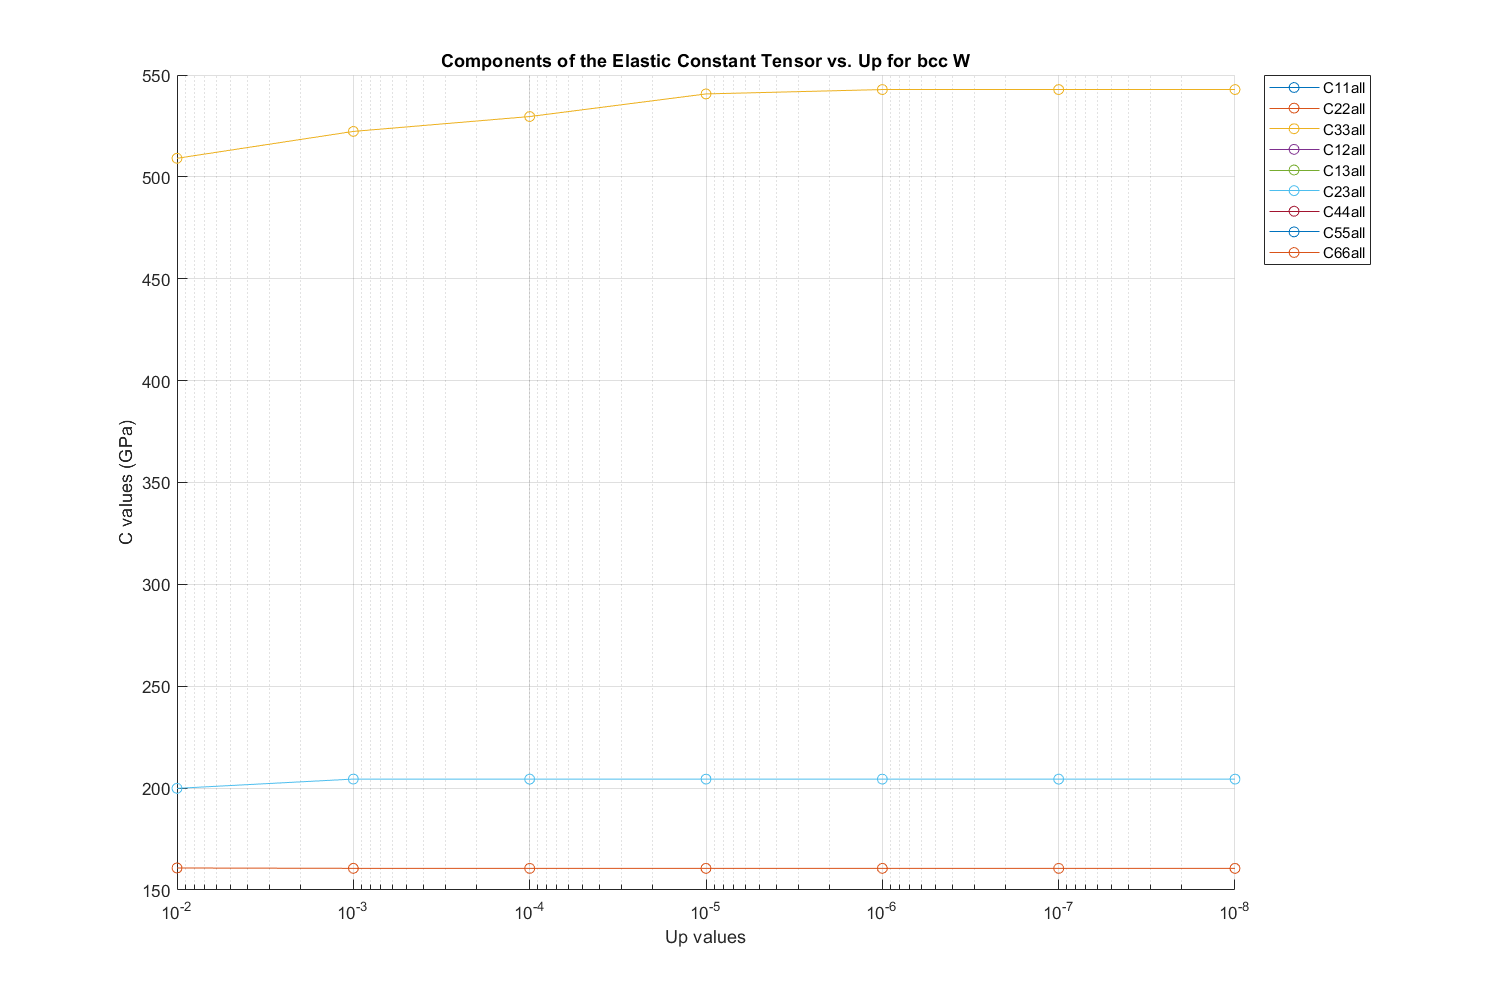
\includegraphics[width=1.1\textwidth]{W.png}
    \caption{Convergence for Components of the Elastic Constant Tensor for bcc W}
\end{figure}
\clearpage
\section*{Conclusion}

\section*{Reference}
[1]: Kittel, C. (2005). Introduction to Solid State Physics (8th ed.). Wiley.
[2]:Yoo, M. H., Lee, J. K., \& Nicholas, T. (1981). Slip, twinning, and fracture in hexagonal close-packed metals. Metallurgical Transactions A, 12(3), 409-418.
[3]:

\end{document}